\documentclass{article}
\usepackage{graphicx}
\usepackage{url}
\usepackage{indentfirst}


\begin{document}

\title{Perceção da Envolvente:}
\maketitle

\section{Introdução}

O nosso projeto tem como principal objetivo tornar o sistemas de cartões da universidade do porto mais sustentável e pratico, atraves de uma carteira digital que permitira aos estudantes e aos funcionarios da universidade do porto utilizarem o seu cartão atraves do telemovel.
Considerando que o nosso publico alvo consistirá na comunidade academica da universidade do porto, decidimos criar e partilhar um inquerito com o objetivo de perceber qual seria a melhor abordagem no desenvolvimento da nossa aplicação.
Ganhando assim conhecimento à cerca das expetativas dos nossos utilzadores sobre a nossa aplicação, assim como o seu à-vontade com as tecnologias e as suas prioridades numa carteira digital.

\section{Análise das respostas}


Obtivemos um total de 48 respostas, todas provenientes de estudantes atualmente matriculados em uma Instituição de Ensino Superior. Considerando o publico alvo previamente defenido isto indica-nos que todas as respostas serão significantes, pois representam possíveis utilizadores da aplicação.

\begin{figure}[h]
    \centering
    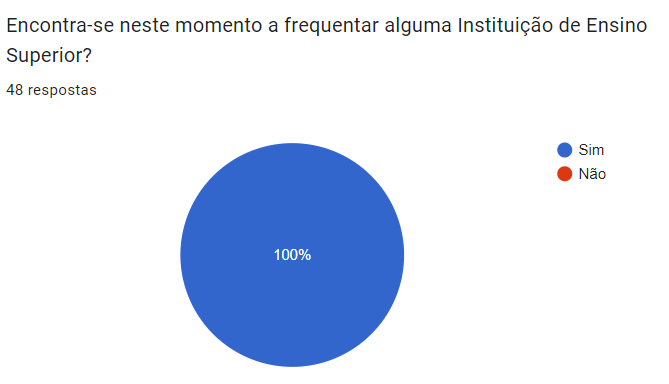
\includegraphics[width=0.7\textwidth]{images/questionaire1.png}
    \caption{Your caption}
\end{figure}


+
\subsection{Frequência e casos de uso}

Cerca de 60\% dos utilizadores responderam que utilizavam o seu cartão institucional com frequência, com os serviços mais utilizados a sendo: \textbf{Acesso à cantina} (~64\%), \textbf{Acesso a salas de aula/núcleos} (50\%) e \textbf{Identificação em testes/exames} (~44\%).
Isto dá nos a entender que será fulcral criar uma aplicação rapidamente acessível para usos pontuais de curta duração, bem como a possibilidade de servir como meio de identificação institucional para o utilizador portador do cartão virtual.

\begin{figure}[h]
    \centering
    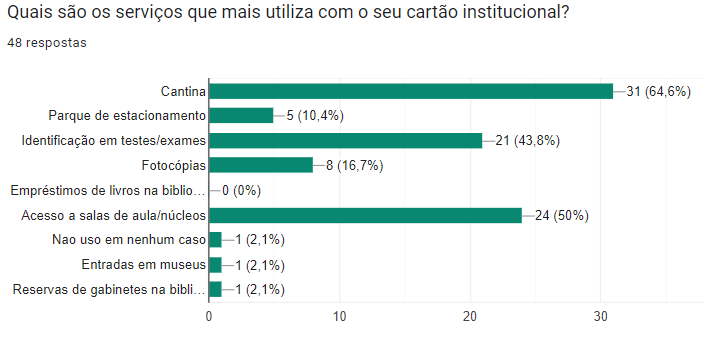
\includegraphics[width=0.9\textwidth]{images/questionaire2.png}
    \caption{Your caption}
\end{figure}

\begin{figure}[h]
    \centering
    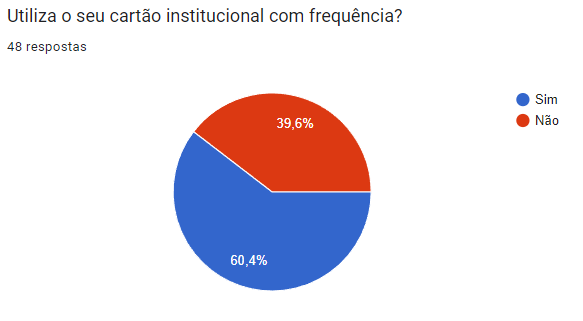
\includegraphics[width=0.9\textwidth]{images/questionaire3.png}
    \caption{Your caption}
\end{figure}

\subsection{Experiência prévia com as tecnologias}

Todos os participantes, à exceção de um, responderam que tinham experiências prévias com cartões virtuais, sendo que, das 47 respostas relevantes, 35 (75\%) relataram uma experiência muito boa na utilização do mesmo. Concluimos assim que o nosso publico alvo sentesse a vontade com as tecnologias usadas, o que nos permitirá usar como inspiração aplicações atuais que implementam estas funcionalidades.
Através do inquerito, também foi nos possivel analisar algumas das dificuldades que alguns participantes tiveram a usar aplicações similares, alguns dessas dificuldades foram:
\begin{itemize}
    \item \textbf Processo de criação do cartão virtual
    \item \textbf Erros na realização das diferentes operações usando a aplicação.
\end{itemize}


Estas dificuldades permite-nos concluir que devemos ter ter cuidado em tornar estes processos intuitivos, e fornecer suporte aos utilizadores.



\subsection{Expectativas e sugestões}

De acordo com as expectativas dos potenciais utilizadores futuros, vemos um maior interesse na segurança da aplicação (77\%) bem como na conveniência que esta trará (71\%). Temos, portanto, de ter um foco em garantir a segurança dos dados dos utilizadores e a coveniência no uso da aplicação que justifique a possível substituição do cartão físico em muitos casos.
Apercebemos-nos também num interesse por uma interface simples para a aplicação (52\%).

\begin{figure}[h]
    \centering
    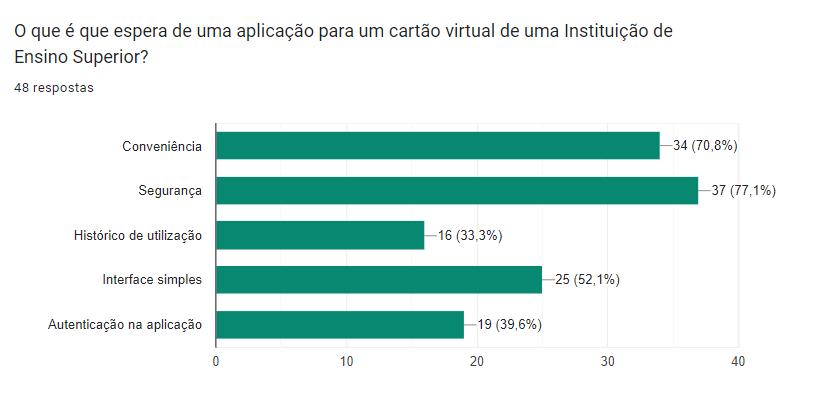
\includegraphics[width=1\textwidth]{images/questionaire4.png}
    \caption{Your caption}
\end{figure}

\end{document}